\section{Meddle Overview}
\label{sec:goals}

In this section, we present an overview of \meddle. We first describe the goals of the 
system, then discuss the \meddle architecture and implementation. 

%\tbd{PG: visibility => VPN which works on all iOSes and across all networks.
%control => Meddle box, with user-enabled SSL bumping, can interpose on all the device traffic.
%deployability => services that users want like device-wide adblock + no reliance on an installed app/the restricted permissions that come along with that. }

\subsection{Goals}

The goals of \meddle are to provide visibility into Internet traffic from mobile devices, 
exert control over this traffic and facilitate a large-scale deployment across multiple 
networks, OSes and devices (smartphones and tablets). We discuss each of these in turn.

%\begin{packeditemize}
%\item 
\noindent\textbf{Visibility}. We aim to capture all of a mobile-device's Internet traffic,
allowing us to characterize network flows and interpose on them using software middleboxes. 
To achieve this, we need a solution that works continuously, regardless of the mobile OS, access 
technology, or apps installed. %Our VPN-based proxy achieves these goals. 
  
\noindent\textbf{Control}. Another important goal is to facilitate research into new middlebox 
applications for mobile traffic. 
It should present a simple API and policy framework for researchers and developers to block, shape, 
inject or otherwise modify network flows matching various criteria. It should also support applications that operate on collections of flows over 
time and across users (\eg Web caching/prefetching, malware detection/blocking and ISP characterization). 


\noindent\textbf{Deployability}. The system must support the ability to deploy and distribute large numbers 
of middlebox services quickly, easily and at scale~\cite{sherry:middleboxes} without 
the need to deploy hardware in homes~\cite{bismark} or ISPs~\cite{wang:middleboxes}. 
To improve the representativeness of studies using \meddle, we want to 
recruit average (\ie non-technical) users to participate in our system. To support this, we need a system 
that has incentives for users, a low barrier to adoption, is easy to deploy and that scales gracefully. 


%\end{packeditemize}
  

\subsection{Architecture \& Implementation}
\begin{figure}[tb]
\centering
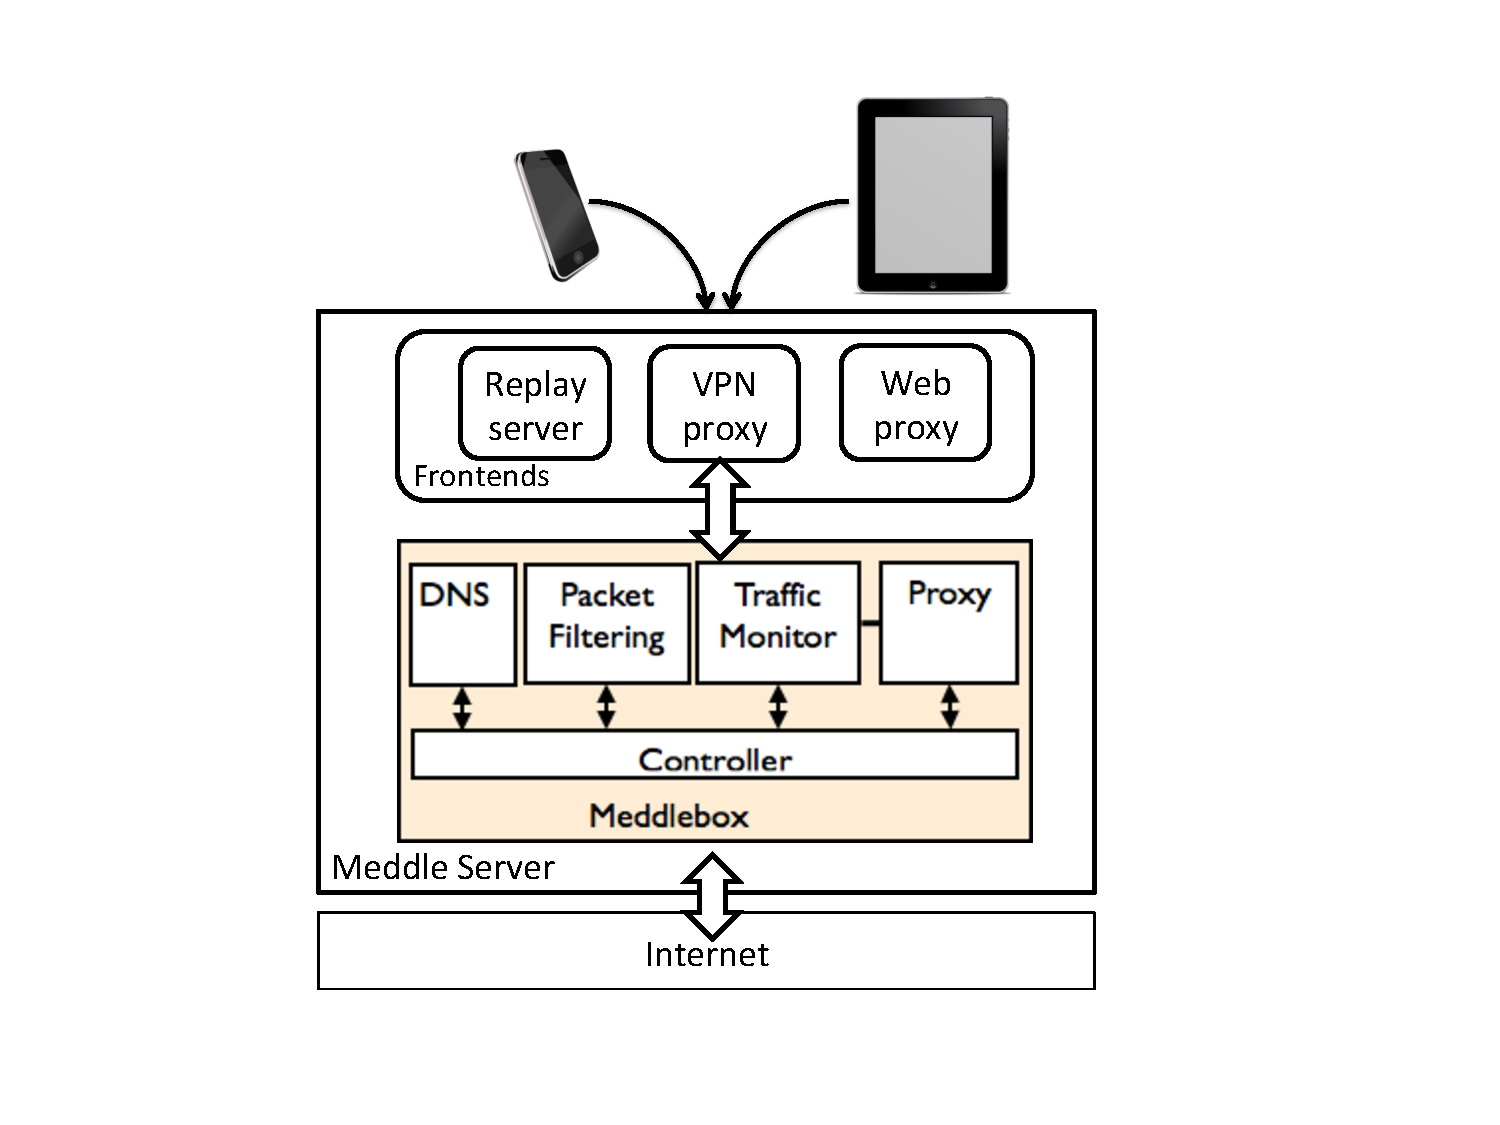
\includegraphics[width=0.8\columnwidth]{figures/meddle-diagram.pdf}
\caption{Architecture for \meddle. Mobile devices (top) communicate with 
a \meddle frontend (VPN proxy, Web proxy and/or 
traffic replay server). VPN proxy traffic is forwarded to a \meddlebox, which provides 
software middlebox services that measure and/or interpose on network flows before 
relaying the traffic to the Internet.  }
\vspace{\postfigspace}
\label{fig:architecture}
\end{figure}

To achieve our goal of visibility, \meddle uses a VPN to direct all of a participating 
mobile device's Internet traffic to a proxy server (top of the Fig.~\ref{fig:architecture}, 
describe in \S\ref{subsec:design_visibility}). To achieve our goal of controlling mobile-device traffic, 
the \meddle proxy directs traffic to a software middlebox, called a \meddlebox (middle of Fig.~\ref{fig:architecture}, described in \S\ref{subsec:design_control}),
that can record, block, modify and/or otherwise interact with mobile-device flows. 
Section~\ref{subsec:design_deploy} describes how we designed \meddle to have clear 
incentives for user adoption and a low barrier to entry to participate.




%%%%%%%

%\meddle attains its goals by exploiting the observation that nearly all devices support network traffic indirection via virtual private networks (VPNs) and HTTP proxies. 
%This network perspective offered by traffic redirection is promising because mobile devices are increasingly becoming the primary gateway to access Internet based services~\cite{ict:facts}. 
%This perspective becomes even more important because a large number of free applications use Internet connectivity with the sole purpose of serving advertisements that make-up for their costs~\cite{pathak:eprof,vallina-rodriguez:bfc}.
%
%
%As depicted in Figure~\ref{fig:architecture}, \meddle relies on a combination of VPN and HTTP based proxies to diagnose traffic from mobile apps and OS services, and to identify ISP interference.
%\meddle uses HTTP proxies, that exchange traffic in the clear, to identify possible ISP interference with HTTP traffic. 
%\meddle uses VPNs to address potential ISP interference, and to diagnose the traffic naturally generated by the mobile apps and OS services.
%
%\meddle's traffic manager determines the flow of the packet, through a combination of VPN and HTTP proxies, before the packet enters the traffic diagnosis engine. 
%On this engine, we deploy a variety of diagnosis tools such as bro. 
%\tbd{Here it must be highlighted that \meddle allows the integration of the existing tools to offer a single platform that can be used for mobile traffic diagnosis. Though simple, it brings with it a power that previously required warranty voiding of devices and ... The novelty lies in exploiting existing features to come up with a feasible user friendly platform}
%
%
%
%VPNs are supported by most mobile OSes\footnote{Android, BlackBerry, and iOS all support VPNs natively, representing more than 86\% of the mobile device market\cite{gartner-phone-share}.} and carriers to satisfy their enterprise clients. 
%Thus \meddle leverages on VPNs for being agnostic to mobile OSes, ISPs, access technologies, and applications used by the mobile device.
%\tbd{what about other goals.. I do not want to put a see section .. here.}
%
%%\subsubsection{Architecture}
%
%\meddle uses VPNs as a portable mechanism to tunnel traffic from mobile devices to a machine outside of the carrier's network for the purpose of analysis and interposition.
%\meddle uses the Squid~\cite{squid} HTTP proxy for two purposes: 1) to monitor the SSL traffic using SSL bumping~\cite{sslbump} which is essentially a man-in-the-middle operation, and 2) inject javascript code inspired by tripwires~\cite{tripwires} to identify ISP interference.
%
%\meddle currently offers the following capabilities to diagnose mobile Internet traffic
%\begin{packedenumerate}
%\item Passive monitoring to characterize the network behavior of application and OS services. 
%\item Enhanced passive monitoring to analyze SSL traffic.
%\item Analysis of ISP interference.
%\item Filtering privacy invasive traffic. 
%\end{packedenumerate}

%\section{System Overview}
%\label{sec:impl}
%We describe the implementation of \meddle, evaluate its performance and discuss 
%the current deployment. We also discuss the benefits and limitations of our approach.

\subsubsection{Visibility: VPN proxying}
\label{subsec:design_visibility}

\meddle leverages the fact that the vast majority of mobile devices provide native VPN support, a feature typically provided to satisfy enterprise clients. We currently support VPN tunnels on iOS and Android; we anticipate being able to support the next version of Windows Phone that includes a native VPN implementation.

\noindent\textbf{iPhone support.} 
All iOS devices (version 3.0 and above) support \textit{VPN On-Demand}, which forces traffic for a specified set of domains to use VPN tunnels. 
This feature is originally intended to allow enterprises to ensure their employees' devices always establish a VPN connection before contacting a specified set of domains. 
To ensure all possible destinations match this list, we exploit the fact that iOS uses suffix matching to determine which connections should be tunneled; accordingly, we specified the domain list as the set of alphanumeric characters (a-z, 0-9, one character per domain). 
To setup this configuration, users need to install a single file, a step that needs to be performed only once. 

\noindent\textbf{Android support.} As of Android 4.2, Android supports ``always on'' VPN connections that ensure all traffic is always tunneled.
For Android version 4.0+ we use a modified StrongSwan implementation of a VPN client app~\cite{strongswanclient}  that 
uses an Android API to manage VPN tunnels. 
Our version ensures re-establishment of VPN tunnels on network state changes (\eg when a device switches from cellular to \wifi).
%\meddle thus supports devices running Android version 4.0 and above.

\noindent\textbf{Server-side implementation.} 
\meddle uses the open-source Strongswan project~\cite{strongswan} to manage the VPN tunnels 
on its servers. When traffic arrives at the server, \meddle uses \emph{tcpdump} and \emph{bro} to record 
traffic via two approaches. One approach captures full packets, 
and requires subjects to be interviewed and provide written informed consent before participating. 
We used this study to inform the second approach, which captures only relevant packet headers 
necessary for the applications we discuss in the remainder in the paper. 

As we described in the previous section, encrypted flows give \meddle no visibility into the 
content of network flows and no ability interpose on that traffic. To regain this visibility, we use SSL 
bumping to decrypt and access the plaintext of encrypted flows in the following way. 
 
First, we note that \meddle's VPN server, like all VPN servers, can be configured to use self-generated root certificate used to sign all subsequent certificates issued to participating mobile devices. 
This allows us to perform SSL traffic decryption using the Squid proxy's SSL bumping~\cite{sslbump} feature.
When the mobile device connects to a services supporting SSL, the proxy masquerades as the service using a forged certificate signed with the \meddle root certificate. 
Then the proxy establishes an SSL connection with the intended target, impersonating a mobile device. 
Using the traffic captured on \meddle and the private key generated by the squid proxy to communicate with the mobile device, we can decrypt all SSL traffic. 
%We note that when traffic is not encrypted using SSL, the proxy simply forwards traffic. 

This approach fails for apps that do not trust certificates signed by unknown root authorities. 
For example, in our controlled experiments we observed that Firefox prevents SSL bumping by validating root certificates, while the Google Chrome, Safari, Facebook, and Google+ apps, as well as the default mail clients and advertisement services, do not check the validity of the root certificate. 
This enables our approach to provide visibility into secure channels established with a wide range of popular apps. 


\subsubsection{Control: Software Middleboxes}
\label{subsec:design_control}
%\begin{figure}
%\begin{center}
%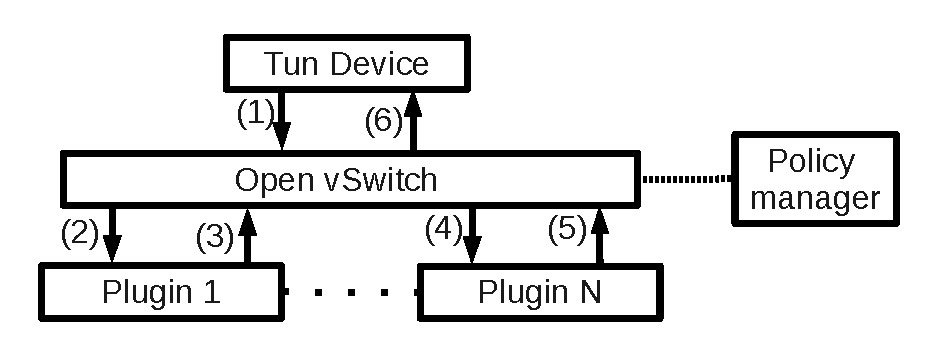
\includegraphics[width=\columnwidth]{figures/packet-monitoring-plugin.pdf}
%\end{center}
%\vspace{\postfigspace}
%\caption{Plugin infrastructure for \platname, which allows traffic to pass through 
%a series of middlebox services before being forwarded to the destination. }
%\label{fig:packet-monitoring-solution}
%\vspace{\postfigspace}
%\end{figure}

Once traffic arrives at a \meddlebox, it interacts with software middleboxes that interpose on 
user-generated traffic and proxy services that interact with 
flows that \meddle induces.  

\noindent\textbf{Plugin infrastructure.}
\platname{} supports a plugin
infrastructure for custom flow processing. Each plugin takes as input a 
network flow and outputs a network flow (potentially empty). 
When a packet arrives at the VPN proxy, \meddle forwards it to a software-defined switch~\cite{Openvswitch} that 
determines the ordered set of plugins that the corresponding flow will traverse. 
This order is configured by a policy manager, which determines 
the set of plugins that should operate on each flow. After the last 
plugin is traversed, \meddle forwards the network flow to the Internet. 
The same approach applies to traffic from the Internet destined for \meddle subscribers. 

Plugins support a variety of features such as ad blocking, 
analyzing PII leakage or page speed optimization. Additionally, we have implemented 
per-connection blocking, malware analysis and DNS-based packet filters. 

\noindent\textbf{Frontend services.} As we describe in \S\ref{sec:isp-behavior}, 
\meddle supports active measurements. 
Specifically, we inject JavaScript into Web pages to detect if the device's 
access network is modifying Web content in flight, and we use a companion app to 
test detect service differentiation within mobile ISPs. To support these, we 
run services on \meddle that are accessed via untunneled connections. 

\subsubsection{Deployability: Incentives and ease of use}
\label{subsec:design_deploy}

%This section describes how \meddle provides clear incentives for user adoption, a 
%low barrier to entry and reasonable performance that is easy to scale.

\mypara{Incentives for user adoption} \meddle presents a number of incentives 
that appeal to a wide range of users. Importantly, we do not charge users for any of these 
services.

%\begin{packeditemize}
\noindent \emph{Improved security.} By securely tunneling all of a mobile device's traffic, users 
are less vulnerable to data leakage (\eg via open WiFi hotspots). 

\noindent \emph{Device-wide content filters.} We use \meddle to block content that users do 
not wish to access -- for all apps running on a device. The most popular instance of this is 
device-wide ad blocking, implemented using a DNS server that returns {\em localhost} for 
requests to names for known ad servers.

\noindent \emph{Privacy revelations~\cite{wetherall:revelations}.} The \emph{ReCon} tool (\S\ref{sec:characterize-app}) allows users to see how they are being 
tracked by ad and analytic servers, and allows them to create per-connection block lists.  

\noindent \emph{ISP transparency.} We provide services that allow users to identify cases where 
ISPs are modifying HTTP content in flight, and when they provide differentiated service to 
traffic crossing their networks (\S\ref{sec:isp-behavior}).

\noindent \emph{Malware detection.} \meddle uses network signatures to identify malware, block it from 
communicating and prevent future downloads onto other \meddle-enabled devices (\S\ref{sec:malware}).  
%\end{packeditemize}

\mypara{Low barrier to entry} 
Configuring a VPN generally requires filling out five fields on an Android phone, and the VPN configuration can be distributed using a single file on iOS. 
%These configurations are primarily required to drive the key exchange algorithms required to establish the VPN tunnels.
We are hosting a cloud-based deployment that is free for users, to support large numbers 
of flows interacting with researcher's {\meddlebox}es. We will make 
the \meddle software publicly available.

For those who want to run their own \meddle instance, 
the \meddle server requires only that a user can run a modern Linux OS with root privileges. This can be deployed 
in a single-machine instance on a home computer, dedicated server or on a VM in the cloud. \meddle is currently in 
private beta with dedicated-server, EC2 and Aliyun deployments in the US, France and China. 


%\end{packedenumerate}

\subsection{Discussion}

\mypara{Limitations} 
%The following technical limitations can impact \meddle's coverage.

%\begin{packeditemize} 
\noindent\emph{Trust.} This paper focuses on a cloud-based \meddle deployment, which requires 
that users trust our system with their network data. We will make our code open source to build this 
trust. For particularly paranoid users, we will also provide a stand-alone implementation that users 
can run on a server of their choice.

\noindent\emph{At most one VPN tunnel.}
Currently iOS and Android support exactly one VPN connection at a time. 
This allows \meddle to measure traffic over either \wifi or cellular interfaces, but not both at once.
The vast majority of traffic uses only one of these interfaces, and VPNs can be used to tunnel that traffic.
%\tbd{MPTCP on iOS 7??}

\noindent\emph{Proxy location.} 
When traffic traverses \meddle, destinations will see the \meddle address, not the device IP, as the source. 
This might impact services  that customize (or block access to) content according to IP address (e.g., in case of localization). 
A solution to this problem is to use a \meddle{} instance with an appropriate IP address.

\noindent\emph{ISP support.}
Some ISPs block VPN traffic, which prevents access to our current \meddle implementation. 
We note that few ISPs block VPN traffic, and there is an incentive not to block VPN traffic to 
support enterprise clients.

\noindent\emph{IPv6.}
\meddle{} cannot be currently used on networks using IPv6; though iOS, Android and StrongSwan support IPv6 
the mobile OSes currently do not support IPv6 traffic through VPN tunnels.
%\end{packeditemize} 


\mypara{Privacy} Our IRB-approved user study reports data from capturing all of a 
subject's Internet traffic, which raises significant privacy concerns.  
The study protocol entails informed consent
from subjects who are interviewed in our lab, where the risks and
benefits of our study are clearly explained.  The incentive to use
\meddle is Amazon.com gift certificates awarded by lottery. To protect the
identity of information leaked in the data, we use public key
cryptography to encrypt all data before storing them 
on disk; the private key is
maintained on separate secure severs and with access limited to
approved researchers.  Further, subjects are free to delete their
data and disable monitoring at any time.  Per the terms of our IRB, we cannot 
make this data publicly available due to privacy concerns. 

Our other IRB-approved \meddle study uses the same protocol except 
for (1) only packet headers are captured, thus reducing the privacy risks, 
and (2) subjects provide electronic informed 
consent, thus facilitating user adoption worldwide. Subjects can sign up at \url{http://meddle.mobi}.

\mypara{Generalizability} A system for improving visibility and control over Internet traffic from mobile 
devices can be implemented at the endpoints (\eg in the OS), in the network (\eg a hardware middlebox), 
somewhere else in the middle (our approach). \meddle is not intended as a blanket replacement for 
these alternative approaches; rather it allows us to explore the opportunities for improving the state of the 
art in today's mobile systems by making mobile Internet traffic available to researchers. 

In some cases, \meddle is the right location to implement new services that could be costly 
to deploy on devices (prefetching) or impractical to deploy in network (detecting ISP service differentiation). 
In other cases, \meddle provides a practical partial solution to a problem where the complete solution has an impractical 
cost. For example, identifying privacy leaks from mobile devices is reliably addressed using information flow 
analysis~\cite{enck:taintdroid}. However, due to the overheads of this approach it is difficult to deploy to users 
and at scale. \meddle allows us to identify and block unobfuscated PII in network flows from arbitrary devices without requiring 
OS modifications or taint tracking. Regardless of the ultimate optimal solution, we can use \meddle today to inform the design 
and deployment of future functionality in OSes and for in-network devices. 


%\noindent\item \textbf{Wi-Fi Gateways powered by Cellular Modems.}


%\subsection{Costs}
%
%\noindent\textbf{Deployment and Running Costs}
%
%\noindent\textbf{Trust Provider}
%
%\subsection{Incentive for Deployment}
%
%\noindent \textbf{Deploy on Home Gateway.}
%This is why we need the single machine constraint. 
%
%\noindent \textbf{Packet Filtering.}
%Custom ad blocks. Protect against data leaks. 
%
%\noindent \textbf{User Interface to Packet Filtering.}
%
%\noindent \textbf{Security from untrusted Wi-Fi APs.}
%
%\subsection{Current Deployment}
%
%\footnote{\meddle is currently in private beta with deployments in the US, France and China. Users sign-up for an IRB approved study through \url{http://meddle.mobi}. We will make the \meddle software publicly available.} 
%
%\subsection{Discussion}




%\noindent \textbf{Modular Architecture for Offloading Activities.}



%%% Local Variables: 
%%% mode: latex
%%% TeX-master: "meddle-main"
%%% End: 
